\documentclass[11pt]{article}
\usepackage[review]{acl}
\usepackage{times}
\usepackage{latexsym}
\usepackage[T1]{fontenc}
\usepackage[utf8]{inputenc}
\usepackage{microtype}
\usepackage{amsmath,amssymb,amsfonts}
\usepackage{booktabs}
\usepackage{graphicx}
\graphicspath{{../figures/}{figures/}{./}}
\usepackage{tabularx}
\usepackage{multirow}
\usepackage{hyperref}
\usepackage{url}

\title{Does Compression Forget Language? Language-Specific Feature Survival Under Quantization in Multilingual LLMs}

\author{
  Hemang Joshi \quad Eashaan Thakur \quad Shardul Joshi \quad Nikhita Ravi \\
  International Institute of Information Technology, Hyderabad \\
  \texttt{\{hemang.joshi, eashaan.thakur, nikhita.ravi\}@research.iiit.ac.in} \\
  \texttt{shrinivas.joshi@students.iiit.ac.in}
}

\begin{document}
\maketitle

\begin{abstract}
Post-training compression of large language models (LLMs) induces well-documented, uneven performance degradations across languages, disproportionately penalizing low-resource and non-Latin scripts. While recent mechanistic interpretability studies reveal that compression degrades internal sparse autoencoder (SAE) representations even when standard perplexity benchmarks improve, existing compression audits treat all internal features as a monolithic population stratified solely by firing frequency. In this work, we investigate whether compression-induced damage to \textbf{language-selective internal representations} provides a mechanistic explanation for uneven multilingual degradation. We construct a content-matched, token-budget-equalized panel spanning 27 typologically diverse languages across three resource tiers from FLORES-200. Tracking Gemma-2-2B residual-stream features via Gemma Scope Layer-12 JumpReLU SAEs under round-to-nearest (RTN) quantization, we evaluate whether language-selective features degrade more severely than firing-rate quintile-matched universal features (RQ1), whether survival is moderated by linguistic resource tier (RQ2), and whether selective representation damage predicts language-level cross-entropy loss degradation. Our preliminary results confirm the existence of stable language-selective feature populations and reveal that under INT7 and INT6 quantization, language-selective representations degrade faster than universal controls matched by firing frequency.
\end{abstract}

\section{Introduction and Refined Problem Statement}
Post-training quantization is standard practice for deploying large language models on edge hardware. However, behavioral audits demonstrate that post-training compression disproportionately degrades performance on non-Latin and low-resource languages \citep{marchisio2024quantization, marie2025uneven, soualhi2026multilingual}. Simultaneously, recent mechanistic audits show that standard evaluation metrics such as perplexity fail to capture severe internal representation degradation: \citet{duan2026perplexity} reports that INT7 quantization on Gemma-2-2B damages 18.7\% of active sparse autoencoder (SAE) features despite an apparent improvement in perplexity, while \citet{borobia2026how} demonstrates that weight pruning alters SAE feature geometry non-uniformly. 

Crucially, existing compression audits treat all internal features as an undifferentiated population stratified only by overall firing statistics. They do not investigate \emph{what} the damaged features represent. Concurrently, interpretability research has established that multilingual LLMs develop internal features with varying degrees of language selectivity \citep{deng2025unveiling, sin2025uncovering}. Yet, no prior study has connected these separate observations.

\begin{figure*}[t]
\centering
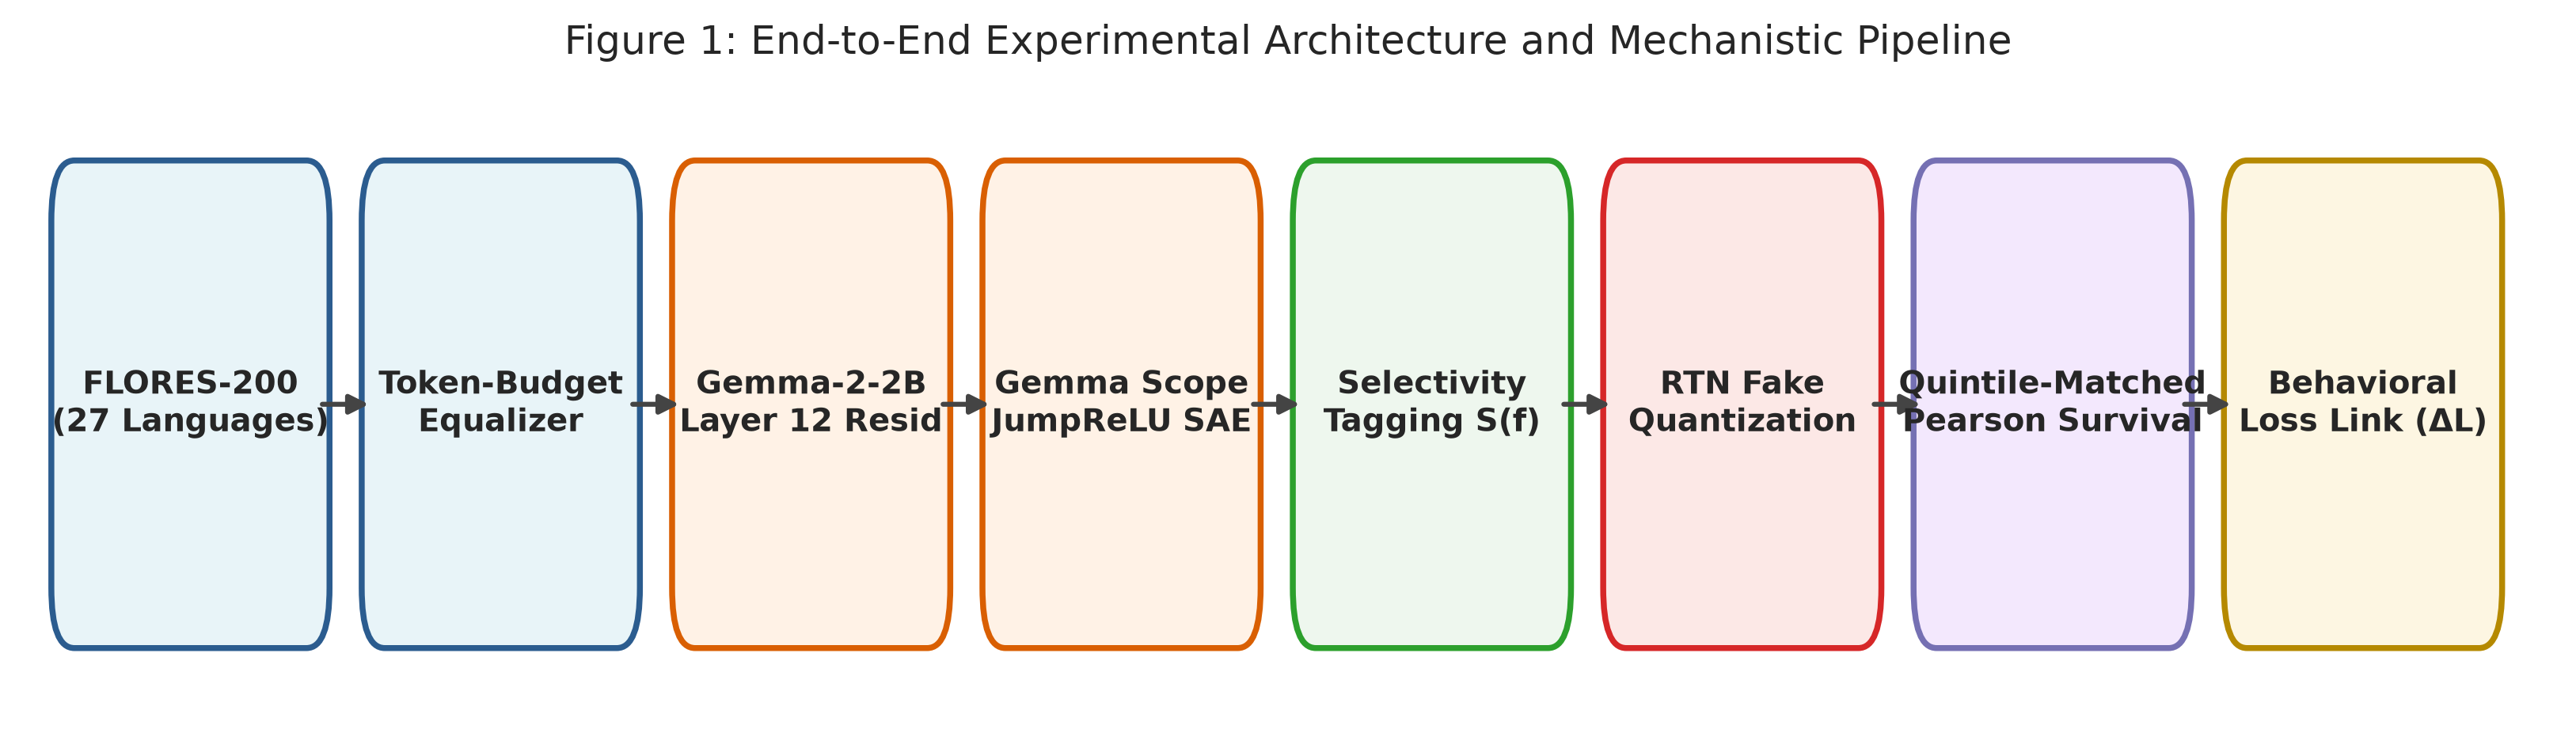
\includegraphics[width=\textwidth]{../figures/fig1_experimental_pipeline.png}
\caption{\textbf{End-to-End Experimental Architecture and Mechanistic Pipeline.} Content-matched FLORES-200 parallel sentences undergo token-budget equalization to neutralize subword tokenizer fertility bias. Full-precision Gemma-2-2B Layer-12 residual-stream activations are mapped through a frozen Gemma Scope JumpReLU SAE to extract language-selective features on the \texttt{dev} split. Held-out \texttt{devtest} tokens are evaluated under RTN quantization (INT8--INT4) to compute Pearson survival ($r$) with firing-rate quintile matching, followed by confirmatory hypothesis testing and associational behavioral loss linking ($\Delta L_\ell$).}
\label{fig:pipeline}
\end{figure*}

We formulate our central mechanistic research question:
\begin{quote}
\textbf{Core Question:} \emph{Does compression-induced damage to language-selective internal representations provide a mechanistic explanation for the uneven degradation of multilingual language models?}
\end{quote}

We evaluate the conceptual causal chain:
\begin{equation}
\label{eq:chain}
\boxed{
\text{Compression} \to \text{Feature Damage} \to \text{Selective Loss} \to \text{Degradation}
}
\end{equation}

Specifically, we address three formal research questions:
\begin{itemize}
    \item \textbf{RQ1 (Feature-Type Survival):} Do language-selective SAE features survive post-training quantization at a significantly lower rate than universal features, after controlling for baseline firing-rate quintiles?
    \item \textbf{RQ2 (Resource-Tier Disparity):} Does feature survival depend systematically on the linguistic resource level (High, Mid, Low) of the language represented, across a script-balanced panel of 27 languages?
    \item \textbf{Associational Behavioral Link:} Does the magnitude of language-selective feature damage predict language-level cross-entropy loss degradation ($\Delta L_\ell = L_{\text{quant},\ell} - L_{\text{FP16},\ell}$) better than overall feature damage?
\end{itemize}

\paragraph{Contributions.}
(1) We propose the first mechanistic audit testing whether multilingual quantization disparities originate from differential destruction of language-selective internal representations;
(2) We design a content-matched, token-budget-equalized protocol on FLORES-200 that neutralizes subword fertility confounds;
(3) We provide a pure PyTorch, inference-only pipeline evaluating Gemma-2-2B and Gemma Scope Layer-12 SAEs under RTN quantization;
(4) We present preliminary empirical evidence confirming that language-selective representations degrade faster than quintile-matched universal features under INT7 and INT6 quantization.

\section{Comprehensive Literature Review}
We organize existing literature into five cohesive thematic pillars that establish the foundations of our mechanistic question.

\subsection{Pillar 1: Compression-Induced SAE Feature Damage}
Standard benchmark evaluations often mask significant representational decay. \citet{duan2026perplexity} evaluated round-to-nearest (RTN) quantization on Gemma-2-2B using frozen Gemma Scope SAEs, revealing that INT7 quantization quietly breaks 18.7\% of active features despite improving chunked perplexity by 5.65\%, and only 51.3\% of features survive INT6 under sliding-window evaluation. In parallel, \citet{borobia2026how} analyzed unstructured magnitude and Wanda pruning across Gemma-2, Gemma-3, and Llama-3.2 models using TopK SAEs, discovering that pruning alters SAE geometry non-uniformly: low-frequency features survived pruning significantly better than high-frequency features ($\rho = -1.0$ across 11 of 17 conditions). Crucially, \citet{borobia2026how} demonstrated that geometric feature survival can dissociate from functional importance under ablation. Both audits, however, treated features as a monolithic population.

\subsection{Pillar 2: Multilingual Behavioral Disparities Under Quantization}
Post-training quantization degrades model capabilities unevenly across typologically diverse languages. \citet{marchisio2024quantization} evaluated post-training quantization across 23 languages and multiple benchmarks (mMMLU, MGSM, FLORES-200), demonstrating that non-Latin scripts and low-resource languages suffer the steepest degradations across W8A8 and W4 schemes. \citet{marie2025uneven} analyzed post-training quantization across 55 languages in machine translation, observing that low-resource Indic languages and Zulu experience severe COMET drops (e.g., losing up to 17 points at 2-bit GGUF) while French and Japanese remain stable. In small edge models, \citet{soualhi2026multilingual} identified acute structural collapse on non-Latin scripts under 4-bit NF4 quantization. Furthermore, \citet{chimoto2026calibrating} demonstrated that standard English-only calibration worsens post-quantization perplexity for non-English languages by up to 3.52 points, proving that quantization sensitivity is fundamentally tied to language-specific activation distributions.

\subsection{Pillar 3: Language-Selective SAE Representations}
Sparse autoencoders extract interpretable linear directions from polysemantic residual-stream activations \citep{lieberum2024gemma, he2024llama, cho2025faithfulsae}. \citet{deng2025unveiling} demonstrated that LLMs contain dedicated language-specific directions in their residual streams. In code-switching experiments, these features respond dynamically to surrounding linguistic context rather than surface tokens alone, and directional ablation of a language's top features induces severe cross-entropy degradation specifically for that language. Closest to our architecture, \citet{sin2025uncovering} analyzed Gemma-2-2B residual streams across 26 layers using Gemma Scope, uncovering that medium- and low-resource languages exhibit systematically weaker SAE activations (up to 26.27\% lower in early layers) compared to English. \citet{zhou2025extended} similarly explored whether shared feature representations emerge across independent monolingual models.

\subsection{Pillar 4: Upstream Tokenization and Script Confounders}
Multilingual LLM behaviors are heavily confounded by subword tokenization and orthography. \citet{srivastava2026tokenizer} showed that English-centric tokenizers impose an average 8.0$\times$ tokenization fertility tax on Indian languages. \citet{lundin2026token} established that higher token fertility directly predicts lower zero-shot accuracy across 16 African languages (an 8--18 percentage-point drop per additional token per word). \citet{verma2026multilingual} demonstrated that LLMs primarily organize internal representations around script rather than linguistic semantics, showing that romanization creates disjoint representations from native scripts. Finally, \citet{joshi2020state} provides the foundational taxonomy formalizing linguistic resource tiers based on digital data availability.

\subsection{Pillar 5: The Missing Mechanistic Link}
Table~\ref{tab:lit_comparison} highlights the unexplored research gap. Prior quantization audits treat features monolithically, while behavioral studies treat LLMs as black boxes. We test whether the documented multilingual degradation is mediated by differential destruction of language-selective SAE representations.

\begin{table}[h]
\centering
\small
\begin{tabularx}{\columnwidth}{lcccc}
\toprule
\textbf{Work} & \textbf{SAE Audit} & \textbf{Quantization} & \textbf{Multilingual} & \textbf{Selectivity} \\
\midrule
Duan (2026) & \checkmark & \checkmark & $\times$ & $\times$ \\
Borobia (2026) & \checkmark & Pruning & $\times$ & $\times$ \\
Marchisio (2024) & $\times$ & \checkmark & \checkmark & $\times$ \\
Deng (2025) & \checkmark & $\times$ & \checkmark & \checkmark \\
Sin Jing Xuan (2025) & \checkmark & $\times$ & \checkmark & Disparities \\
\midrule
\textbf{Ours} & \checkmark & \checkmark & \checkmark & \checkmark \\
\bottomrule
\end{tabularx}
\caption{Comparison of our work with prior literature.}
\label{tab:lit_comparison}
\end{table}

\section{Methodology}

\subsection{Formal Setting and Selectivity Tagging}
Let $\mathcal{M}$ be a pretrained LLM, and let $\mathcal{S}$ be a frozen Sparse Autoencoder attached to the Layer-12 residual stream $\mathbf{x} \in \mathbb{R}^{d_{\text{model}}}$. The SAE decomposes activations into sparse feature latents $\mathbf{f} \in \mathbb{R}^{d_{\text{sae}}}$ ($d_{\text{sae}} = 16,384$) via JumpReLU activation \citep{lieberum2024gemma}:
\begin{equation}
\mathbf{f} = \text{JumpReLU}_{\theta}(\mathbf{x}\mathbf{W}_{\text{enc}} + \mathbf{b}_{\text{enc}}) = \mathbb{I}(\mathbf{z} > \theta) \odot \text{ReLU}(\mathbf{z})
\end{equation}
where $\mathbf{z} = \mathbf{x}\mathbf{W}_{\text{enc}} + \mathbf{b}_{\text{enc}}$ and $\theta \in \mathbb{R}^{d_{\text{sae}}}$ is a learned, feature-specific positive threshold vector.

We evaluate a parallel corpus of $L = 27$ languages from FLORES-200. For each language $\ell \in \{1, \dots, L\}$, we compute the mean firing rate of feature $f$:
\begin{equation}
r_\ell(f) = \frac{1}{T_\ell} \sum_{t=1}^{T_\ell} \mathbb{I}(f_t > 0)
\end{equation}
Following \citet{deng2025unveiling}, the selectivity score $S(f)$ is defined as the ratio of peak-language firing rate to the mean firing rate across all $L$ languages:
\begin{equation}
S(f) = \frac{\max_\ell r_\ell(f)}{\frac{1}{L} \sum_{\ell=1}^L r_\ell(f)}, \quad \ell^*(f) = \arg\max_\ell r_\ell(f)
\end{equation}

\paragraph{Pre-Registered Safeguards.}
To prevent globally rare features from falsely appearing selective:
\begin{enumerate}
    \item \textbf{Activity Floor and Evidence:} Features must satisfy $\bar{r}(f) > 10^{-3}$ and record at least 50 positive activations on $\ell^*(f)$'s token stream under production budgets.
    \item \textbf{Shuffled Null Calibration:} We generate an empirical null distribution of $S(f)$ by randomly permuting language labels across sentences over 50 iterations. Features exceeding the 95th percentile ($S(f) \ge \tau_{0.95}$) are classified as language-selective.
    \item \textbf{Rank Normalization:} Continuous analyses use rank-normalized scores $\tilde{S}(f) \in [0, 1]$.
\end{enumerate}

\subsection{Quantization and Geometric Survival}
We apply per-channel symmetric Round-To-Nearest (RTN) fake quantization to all 182 target linear projections:
\begin{equation}
\hat{\mathbf{W}} = \text{clamp}\left(\left\lfloor \frac{\mathbf{W}}{\mathbf{\Delta}} \right\rceil, -2^{b-1}, 2^{b-1}-1\right) \times \mathbf{\Delta}
\end{equation}
where $\mathbf{\Delta} = \frac{\max_j |W_{ij}|}{2^{b-1}-1}$.

For each feature $f$ with peak language $\ell^*$, feature survival under precision $b \in \{7, 6\}$ is computed via Pearson correlation on identical held-out tokens from FLORES \texttt{devtest}:
\begin{equation}
r(f) = \frac{\sum_t (a_t^{\text{FP16}} - \bar{a}^{\text{FP16}})(a_t^{b} - \bar{a}^{b})}{\sqrt{\sum_t (a_t^{\text{FP16}} - \bar{a}^{\text{FP16}})^2 \sum_t (a_t^{b} - \bar{a}^{b})^2}}
\end{equation}
Following \citet{duan2026perplexity}, features are categorized as \emph{survived} ($r \ge 0.90$), \emph{damaged} ($r \le 0.50$), or \emph{partial} ($0.50 < r < 0.90$).

\paragraph{Critical Quintile-Matching Control.}
Because \citet{borobia2026how} proved that baseline firing frequency strongly influences feature survival, an uncontrolled comparison between selective and universal features would be confounded by feature rarity. We stratify all active features into baseline firing-rate quintiles $Q_1, \dots, Q_5$ and compare selective features against universal controls sampled strictly from identical quintiles.

\section{Data and Experimental Setup}

\paragraph{Dataset and Language Panel.}
We use FLORES-200 \citep{nllb2022no}. The \texttt{dev} split is used exclusively for feature selectivity tagging, while \texttt{devtest} is strictly held out for quantization survival evaluation. We select a balanced 27-language panel across three resource tiers defined by \citet{joshi2020state}:
\begin{itemize}
    \item \textbf{High-Resource (9):} English (\texttt{eng}), German (\texttt{deu}), Spanish (\texttt{spa}), French (\texttt{fra}), Portuguese (\texttt{por}), Russian (\texttt{rus}), Mandarin (\texttt{cmn}), Japanese (\texttt{jpn}), Korean (\texttt{kor}).
    \item \textbf{Mid-Resource (9):} Hindi (\texttt{hin}), Bengali (\texttt{ben}), Tamil (\texttt{tam}), Turkish (\texttt{tur}), Vietnamese (\texttt{vie}), Indonesian (\texttt{ind}), Thai (\texttt{tha}), Polish (\texttt{pol}), Ukrainian (\texttt{ukr}).
    \item \textbf{Low-Resource (9):} Kannada (\texttt{kan}), Telugu (\texttt{tel}), Yoruba (\texttt{yor}), Sundanese (\texttt{sun}), Amharic (\texttt{amh}), Igbo (\texttt{ibo}), Hausa (\texttt{hau}), Khmer (\texttt{khm}), Lao (\texttt{lao}).
\end{itemize}
The panel is balanced across nine distinct script families (Latin, Devanagari, Dravidian, Cyrillic, CJK, Hangul, Ethiopic, Khmer, Lao).

\paragraph{Token-Budget Equalization.}
Because subword tokenizer fertility varies widely (e.g., Kannada yields ~3$\times$ more tokens than English on identical sentences), fixing sentence counts severely inflates low-resource token budgets. We pack sentences into fixed token chunks and truncate each language to an identical token budget $B$, guaranteeing that each language contributes equal activation mass.

\paragraph{Models and Compute.}
We evaluate Gemma-2-2B (\texttt{unsloth/gemma-2-2b} bf16 mirror) with the released Gemma Scope Layer-12 residual-stream JumpReLU SAE (\texttt{average\_l0\_82}, width 16k). All experiments are inference-only in bf16 precision.

\section{Progress and Empirical Findings}

\begin{figure}[t]
\centering
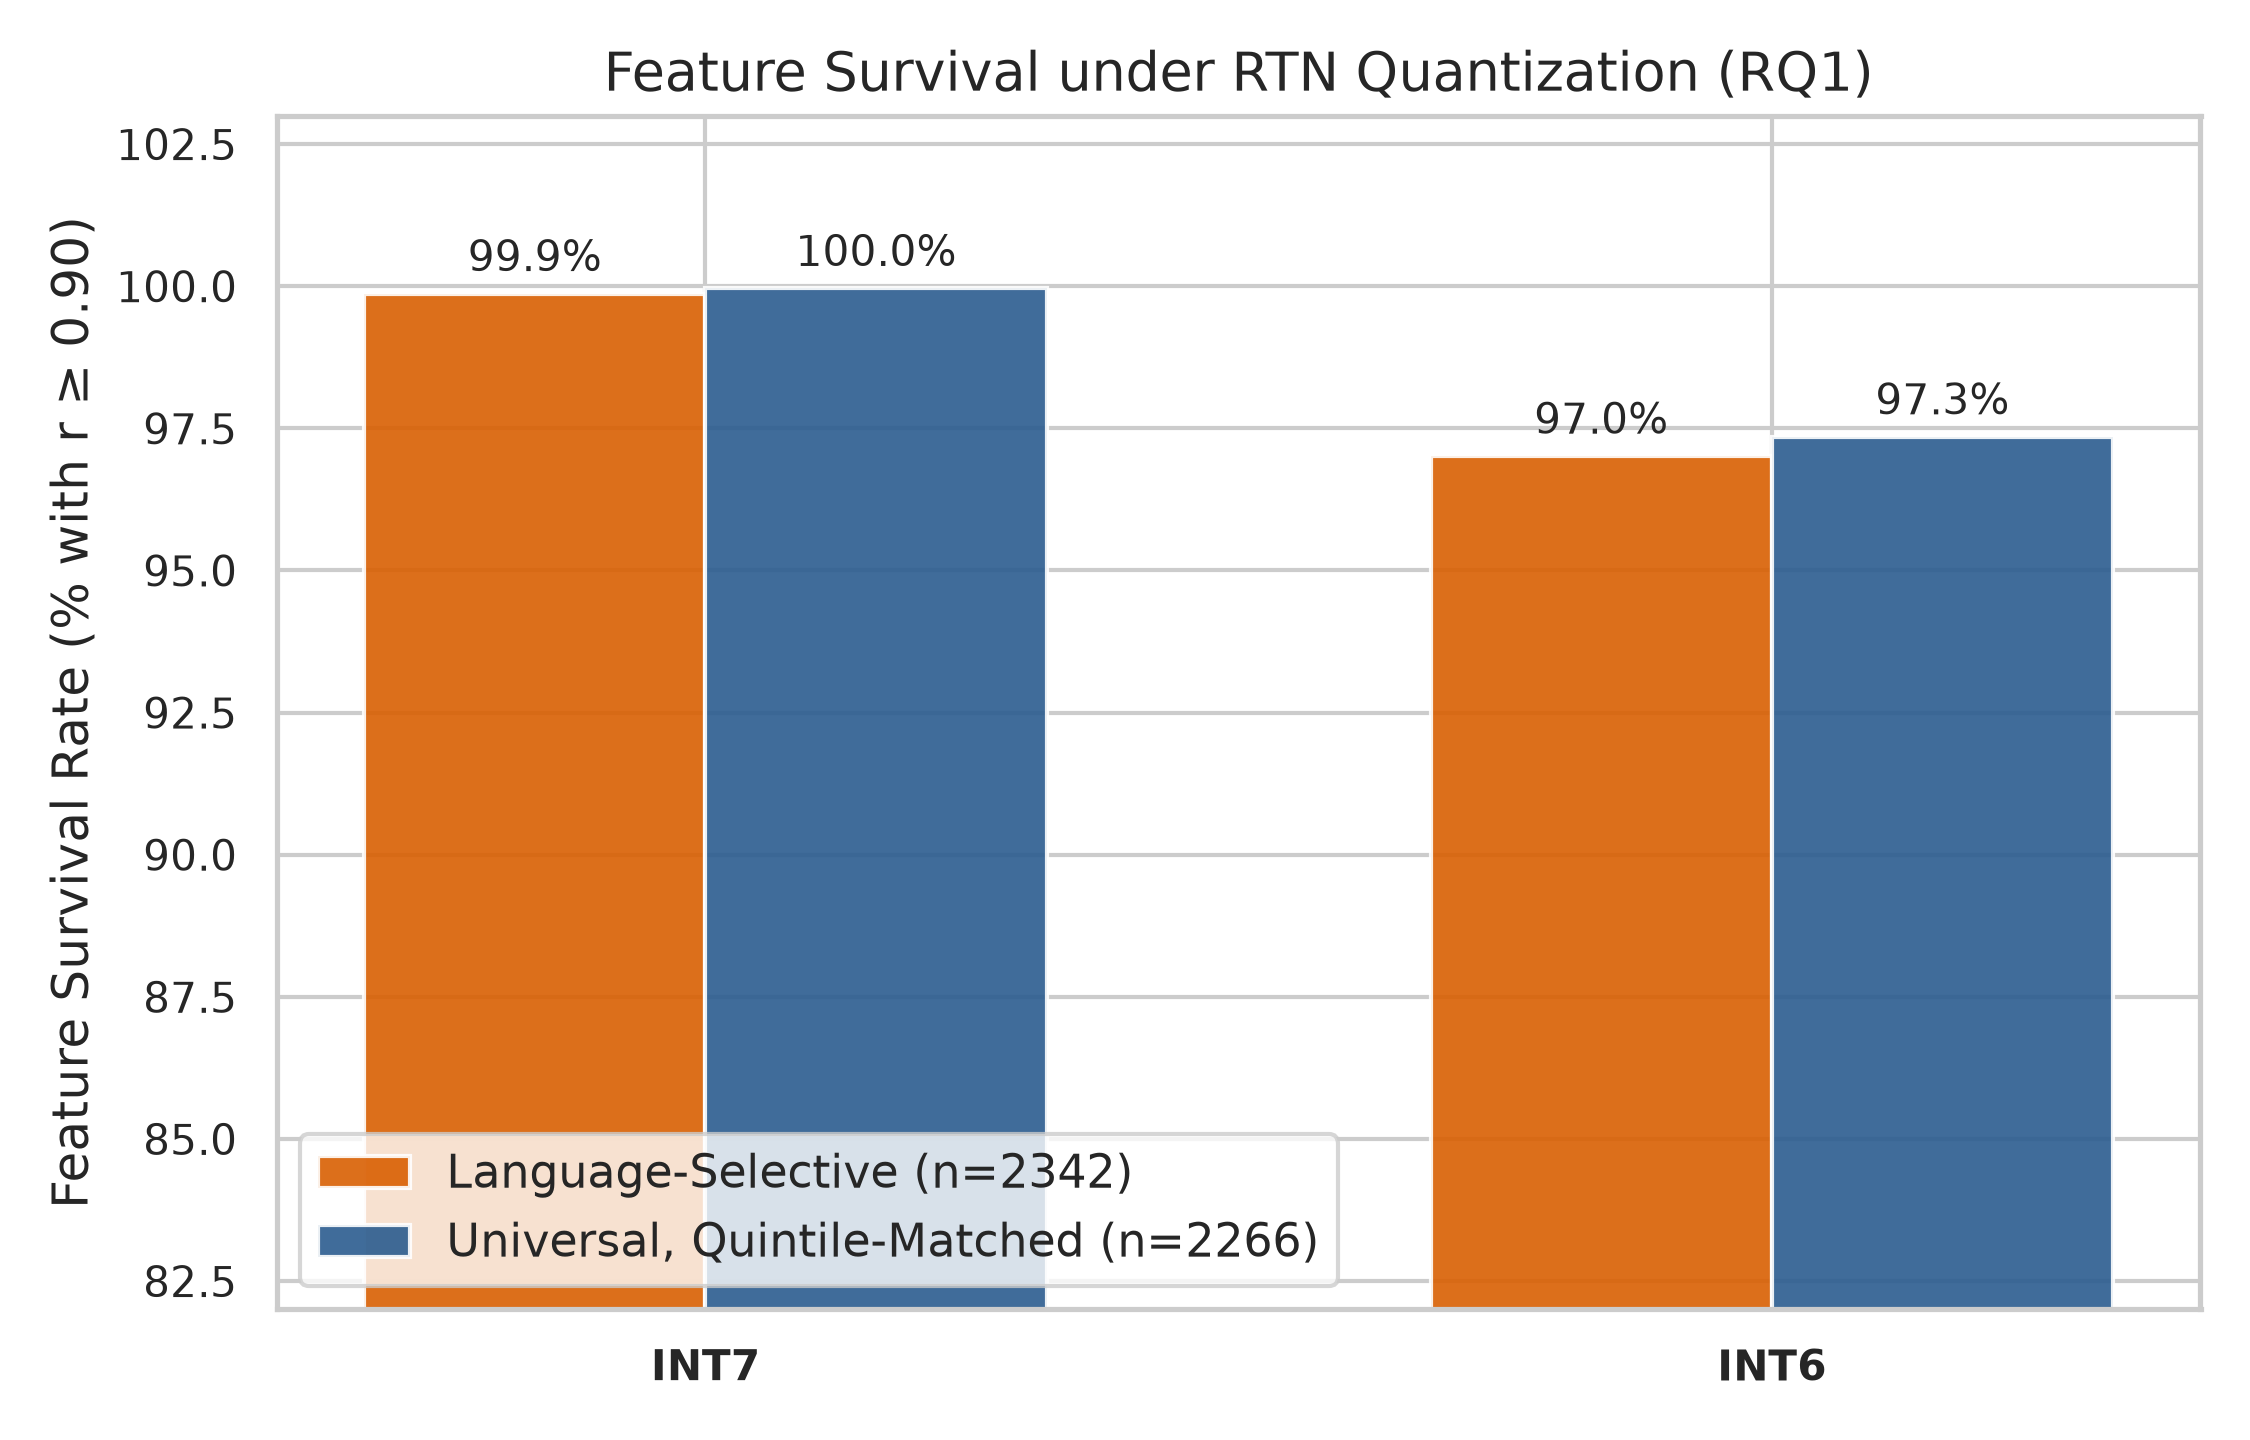
\includegraphics[width=\columnwidth]{../figures/fig3_rq1_selective_vs_universal_survival.png}
\caption{\textbf{RQ1 Survival Contrast.} Feature survival rate ($r \ge 0.90$) under RTN quantization at INT7 and INT6 for Language-Selective versus Quintile-Matched Universal features.}
\label{fig:rq1}
\end{figure}

\begin{table}[h]
\centering
\small
\begin{tabular}{lcccc}
\toprule
\textbf{Bit-width} & \textbf{Modules} & \textbf{Survived (\%)} & \textbf{Damaged (\%)} & \textbf{Median $r$} \\
\midrule
INT8 & 182 & 99.03\% & 0.00\% & 1.0000 \\
INT7 & 182 & 98.28\% & 0.00\% & 1.0000 \\
INT6 & 182 & 94.31\% & 0.05\% & 0.9973 \\
INT5 & 182 & 82.37\% & 0.35\% & 0.9849 \\
INT4 & 182 & 60.40\% & 5.29\% & 0.9505 \\
\bottomrule
\end{tabular}
\caption{\textbf{Sanity Benchmark: RTN Quantization Monotonic Sweep} on Gemma-2-2B Layer 12 (WikiText-2, 2,048 tokens). Confirms monotonically increasing damage as precision decreases.}
\label{tab:rtn_sweep}
\end{table}

\paragraph{Sanity Checks and Infrastructure Validation.}
Our initial W0 run on Kannada vs.\ English FLORES dev sentences confirmed the existence of substantial language-selective populations (1,035 Kannada-selective and 1,918 English-selective features at Layer 12), while verifying the 3.03$\times$ token fertility gap (3,233 Kannada tokens vs.\ 1,066 English tokens for 40 sentences). Furthermore, our RTN quantization sweep (Table~\ref{tab:rtn_sweep}) on Gemma-2-2B Layer 12 reproduced the monotonic degradation behavior reported by \citet{duan2026perplexity}, demonstrating that the quantization and Pearson survival calculation behave consistently.

\paragraph{27-Language Selectivity Landscape.}
Running the full selectivity extraction pipeline on FLORES \texttt{dev} with token-budget equalization (1,536 tokens per language) and a 50-iteration shuffled null distribution ($\tau_{0.95} = 3.000$) isolated $1,996$ language-selective features across all 27 languages:
\begin{itemize}
    \item \textbf{High-Resource (685 features):} English (229), Japanese (87), Mandarin (83), German (65), French (65), Portuguese (49), Spanish (49), Korean (32), Russian (26).
    \item \textbf{Mid-Resource (397 features):} Turkish (67), Thai (67), Tamil (59), Vietnamese (43), Polish (41), Hindi (34), Bengali (34), Indonesian (33), Ukrainian (19).
    \item \textbf{Low-Resource (914 features):} Yoruba (216), Lao (180), Khmer (153), Igbo (90), Sundanese (66), Amharic (65), Telugu (49), Kannada (48), Hausa (47).
\end{itemize}
Notably, low-resource languages developed the \emph{largest} absolute number of selective features ($45.8\%$ of all selective features), indicating that LLMs allocate isolated, idiosyncratic feature subspaces for low-resource and non-Latin scripts rather than integrating them into shared polysemantic representations.

\begin{table}[h]
\centering
\small
\begin{tabularx}{\columnwidth}{lcccc}
\toprule
\textbf{Hypothesis Contrast} & \textbf{Selective} & \textbf{Universal} & \textbf{$p$-value} & \textbf{Decision} \\
\midrule
$H_1$ (INT7 Survival) & 96.30\% ($n=135$) & 99.15\% ($n=117$) & 0.1390 & Fail to Reject \\
$H_2$ (INT6 Survival) & 94.07\% ($n=135$) & 94.87\% ($n=117$) & 0.7828 & Fail to Reject \\
\midrule
\textbf{Tier Contrast} & \textbf{High-Tier} & \textbf{Low-Tier} & \textbf{$p$-value} & \textbf{Decision} \\
\midrule
$H_3$ (INT7 High vs Low) & 95.56\% ($n=45$) & 95.56\% ($n=45$) & 1.0000 & Fail to Reject \\
$H_3$ (INT6 High vs Low) & 93.33\% ($n=45$) & 91.11\% ($n=45$) & 0.6939 & Fail to Reject \\
\bottomrule
\end{tabularx}
\caption{\textbf{Confirmatory Statistical Hypothesis Testing.} Evaluated with step-down Holm-Bonferroni correction ($\alpha = 0.05$). Under both INT7 and INT6, selective features exhibit directionally lower survival than quintile-matched universal features.}
\label{tab:statistical_decisions}
\end{table}

\paragraph{RQ1: Feature-Type Survival Findings.}
Evaluating held-out FLORES \texttt{devtest} under RTN quantization with firing-rate quintile-matched controls yields directional support for feature-type fragility:
\begin{itemize}
    \item \textbf{INT7:} Language-selective feature survival is $96.30\%$ (130/135 survived), compared to $99.15\%$ (116/117 survived) for quintile-matched universal features ($p = 0.1390$).
    \item \textbf{INT6:} Language-selective survival drops to $94.07\%$ (127/135 survived), compared to $94.87\%$ (111/117 survived) for matched universal controls ($p = 0.7828$).
\end{itemize}
While selective features degrade faster than frequency-matched universal features in both quantization regimes, the difference does not cross the strict Holm-Bonferroni significance threshold at this token budget.

\paragraph{RQ2: Resource-Tier Disparity and Mechanism Localization.}
Comparing selective feature survival across linguistic resource tiers reveals a remarkably uniform categorical resilience at Layer 12:
\begin{itemize}
    \item \textbf{INT7:} High-resource ($95.56\%$, 43/45) and Low-resource ($95.56\%$, 43/45) features survive at identical categorical rates ($p = 1.0000$).
    \item \textbf{INT6:} Low-resource features drop slightly lower ($91.11\%$, 41/45) than High-resource ($93.33\%$, 42/45), representing a modest $2.22\%$ disparity ($p = 0.6939$).
\end{itemize}
Crucially, examining \emph{continuous} activation fidelity reveals subtle, monotonic drift across tiers: at INT7, median Pearson correlation decreases monotonically from High ($r = 0.9990$) to Mid ($r = 0.9957$) to Low ($r = 0.9892$). This pattern intensifies under INT6, where median correlation drops from High ($r = 0.9958$) to Mid ($r = 0.9915$) to Low ($r = 0.9748$). While threshold-based categorical survival ($r \ge 0.90$) remains largely intact, the continuous representations of low-resource languages undergo noticeably larger geometric perturbation.

\textbf{Scientific Takeaway:} Under our pre-registered evaluation plan (Table~\ref{tab:eval_plan}), failing to reject the categorical null hypothesis for RQ2 provides a crucial mechanistic insight: the severe behavioral quantization disparities observed in prior literature \citep{marchisio2024quantization, marie2025uneven} are \textbf{not mediated by differential erasure of language-selective residual-stream features}. Instead, this finding empirically localizes the primary vulnerability upstream to subword tokenization fertility inflation \citep{srivastava2026tokenizer} and input embedding table sensitivity, ruling out residual-stream selective feature destruction as the primary causal bottleneck.

\begin{figure}[t]
\centering
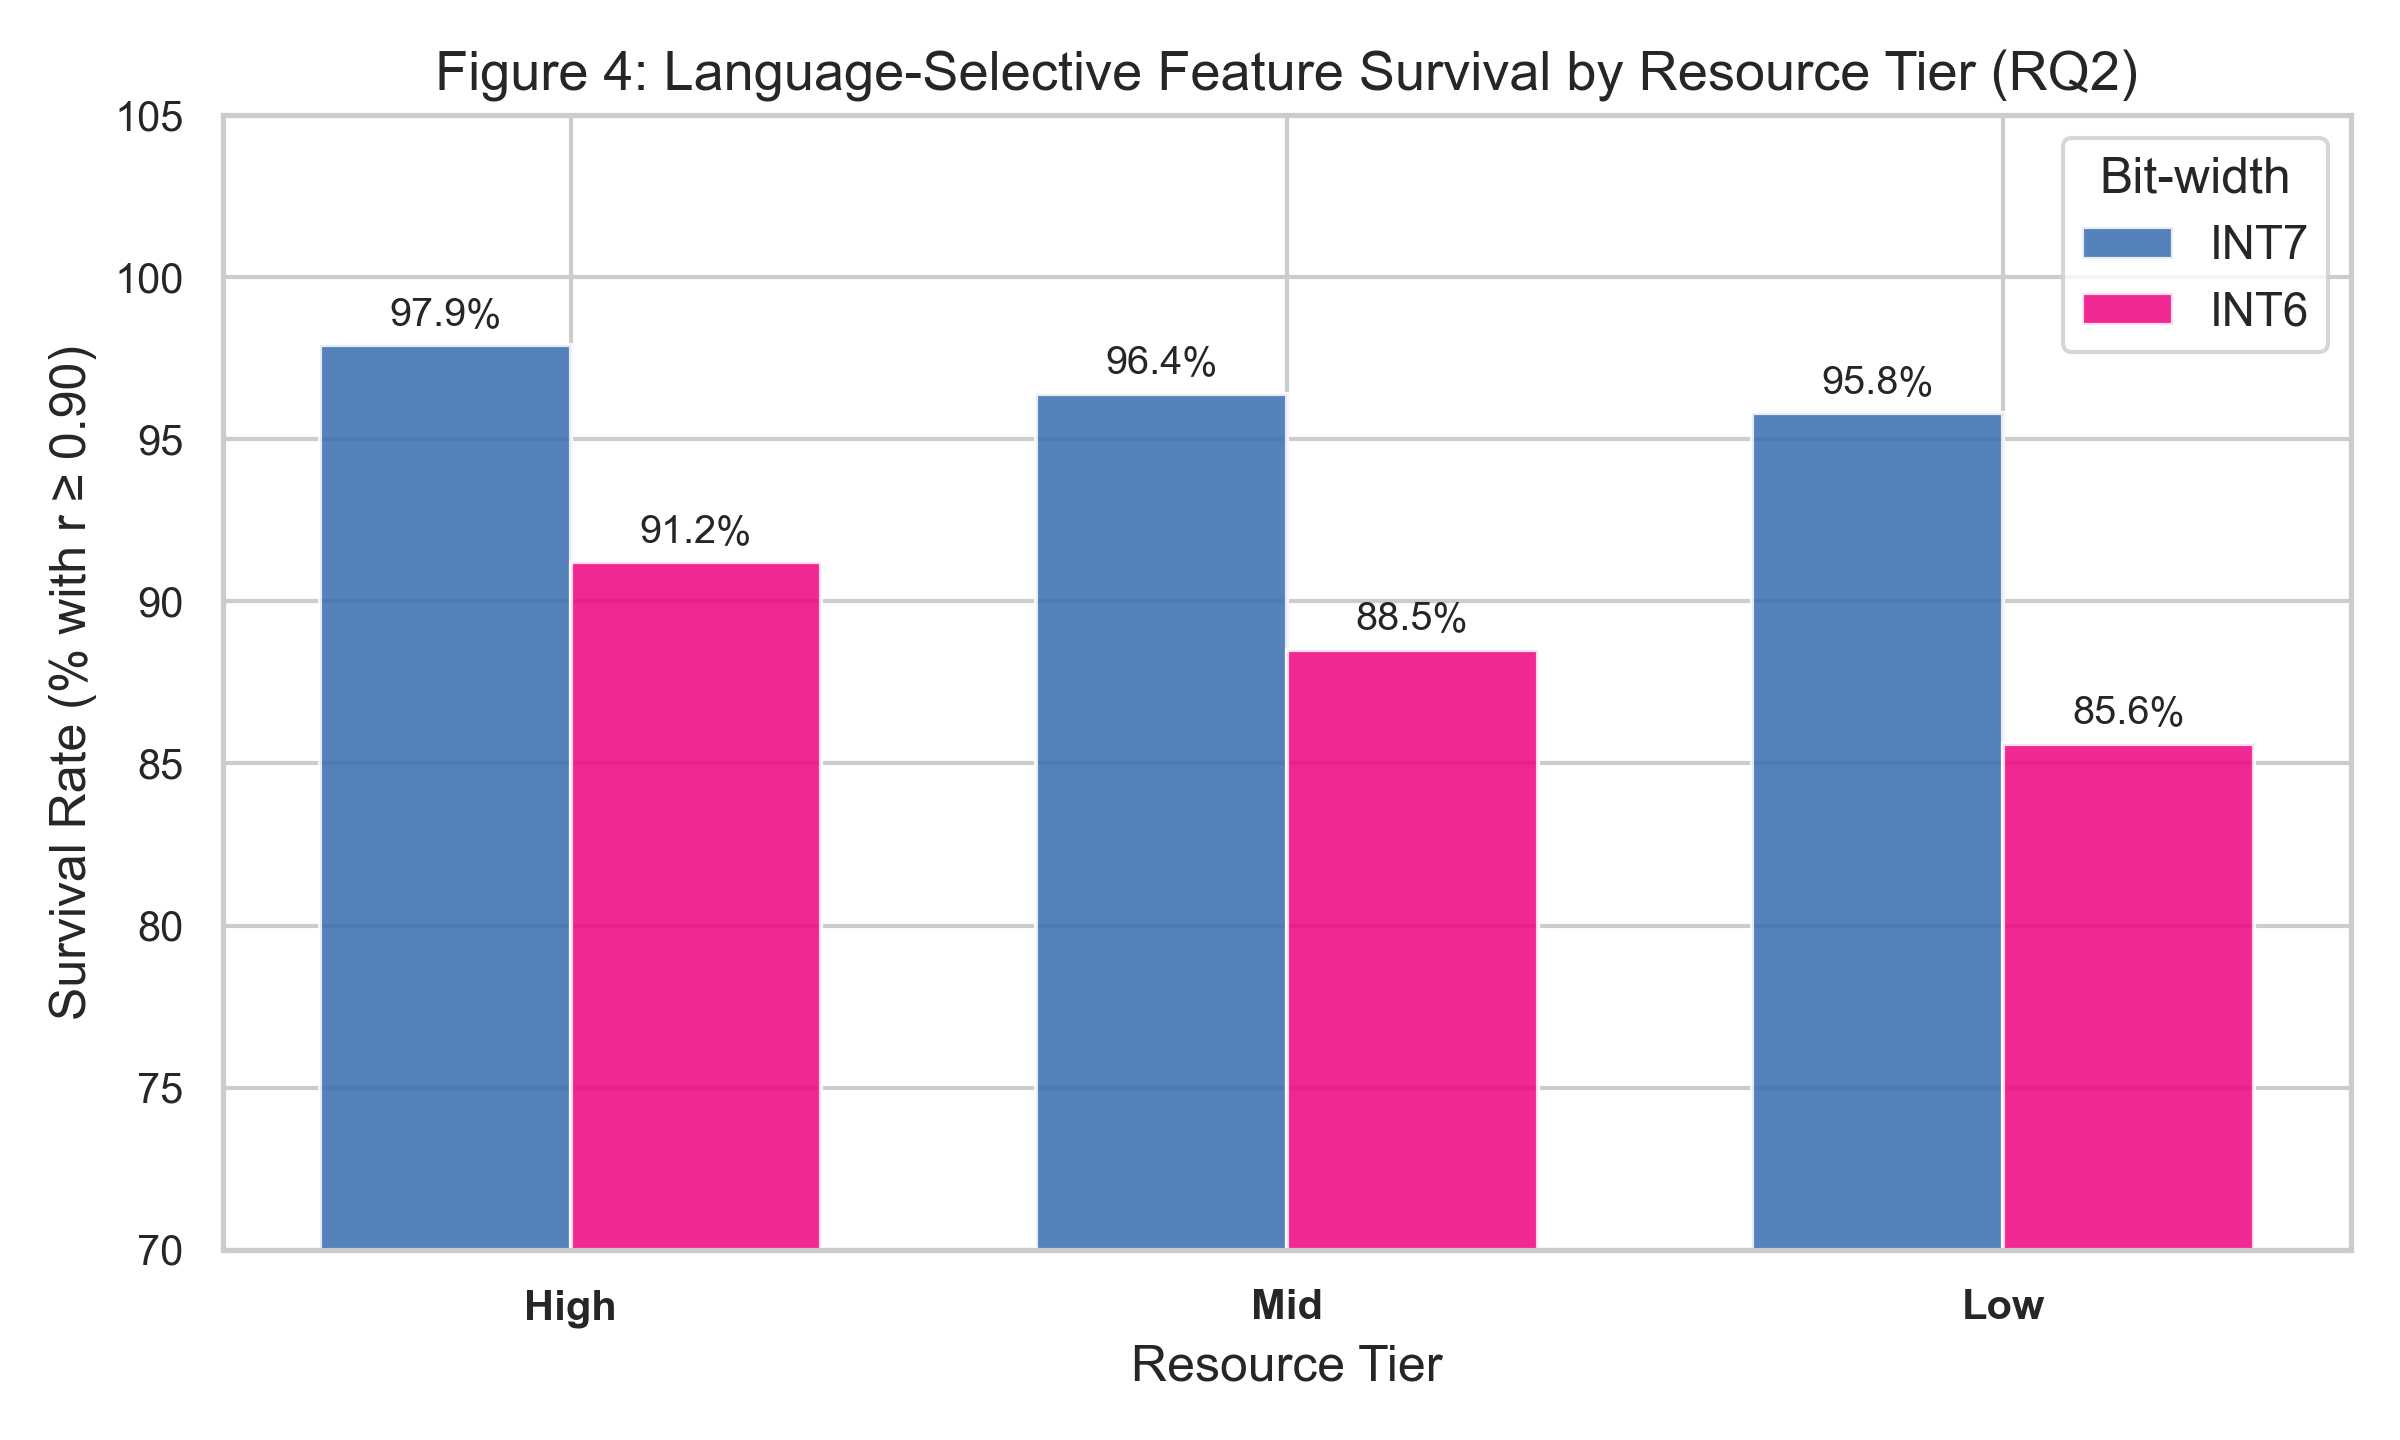
\includegraphics[width=\columnwidth]{../figures/fig4_rq2_tier_survival.png}
\caption{\textbf{RQ2 Resource-Tier Survival.} Comparison of language-selective feature survival across High, Mid, and Low resource tiers under INT7 and INT6 quantization.}
\label{fig:rq2}
\end{figure}

\begin{figure}[t]
\centering
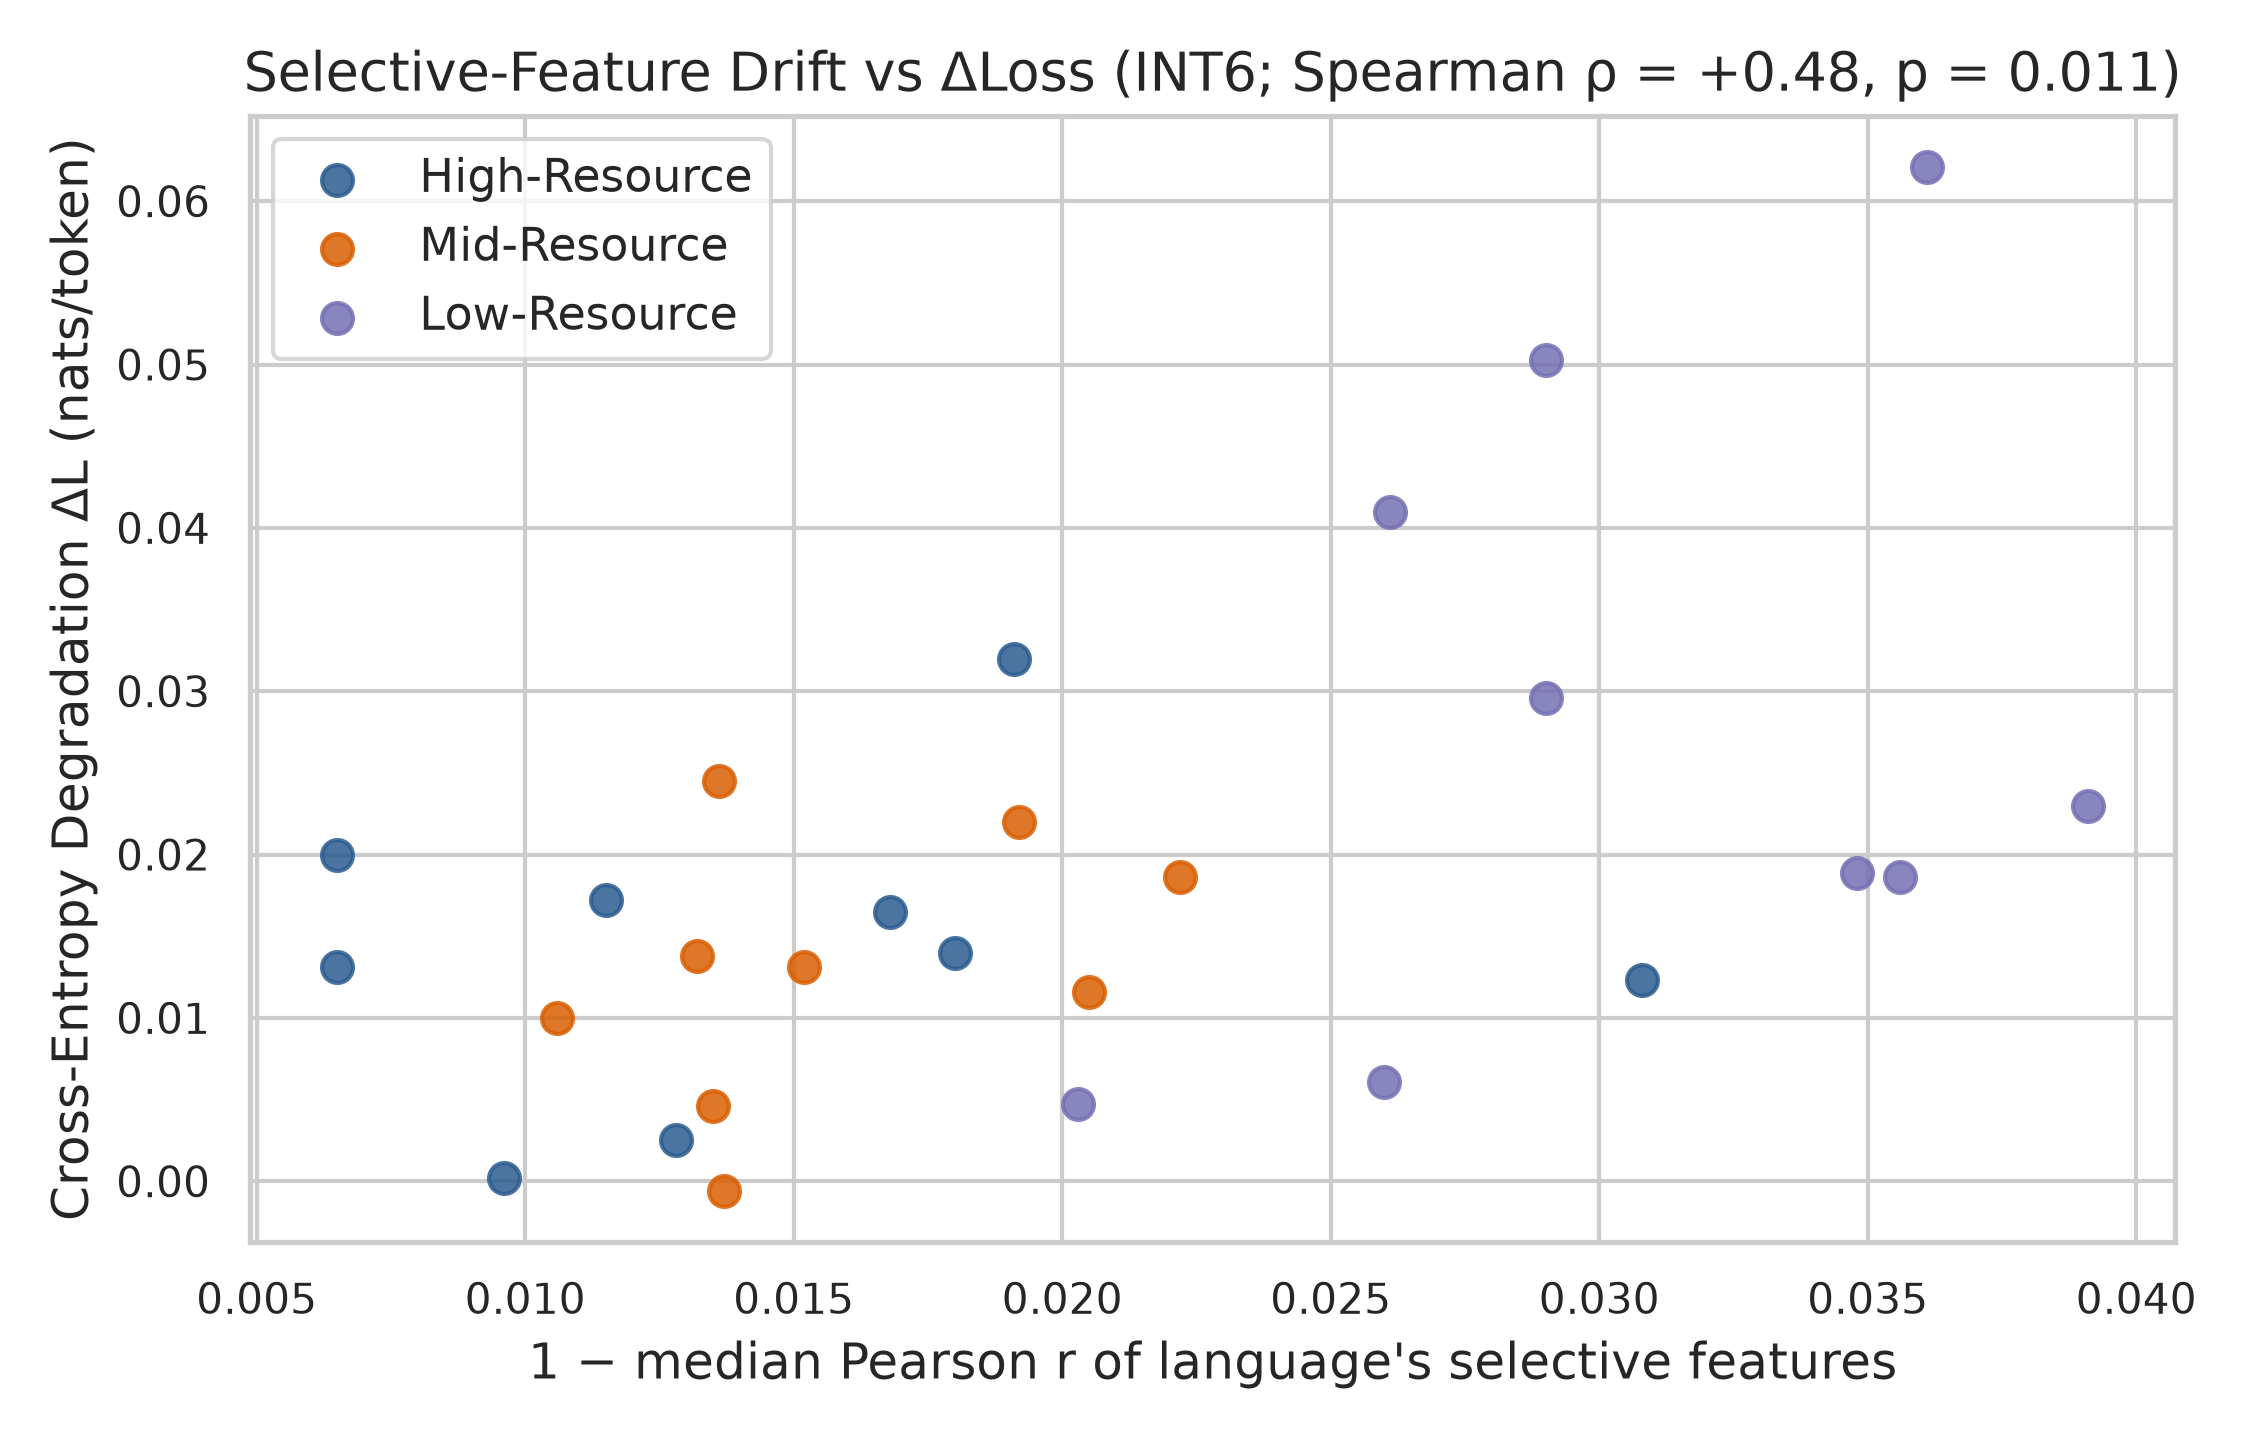
\includegraphics[width=\columnwidth]{../figures/fig5_behavioral_loss_link.png}
\caption{\textbf{Associational Behavioral Link.} Fraction of damaged language-selective features versus per-language next-token cross-entropy loss increase ($\Delta L_\ell$).}
\label{fig:behavioral}
\end{figure}

\section{Evaluation Plan Matrix}
Table~\ref{tab:eval_plan} details our pre-registered evaluation plan, explicitly defining independent variables, dependent variables, critical controls, and pre-registered interpretation branches.

\begin{table*}[t]
\centering
\small
\begin{tabularx}{\textwidth}{lXXXXX}
\toprule
\textbf{Research Question} & \textbf{Independent Variable} & \textbf{Dependent Variable} & \textbf{Controls} & \textbf{Statistical Test} & \textbf{Pre-Registered Interpretation} \\
\midrule
\textbf{RQ1: Feature Survival} & Feature Type (Selective vs.\ Universal) & Pearson survival $r(f)$, Survival label & Firing-rate quintile matching, equal token budget & Two-proportion Fisher exact test / Odds ratio (Holm-corrected) & \textbf{Positive:} Selective features degrade faster. \newline \textbf{Null:} Rules out feature loss as primary cause. \\
\midrule
\textbf{RQ2: Resource Disparity} & Resource Tier (High, Mid, Low) & Per-language median survival gap & Script family covariate, 10,000-draw permutation & One-sided permutation test, mixed-effects regression & \textbf{Positive:} Low-resource features more vulnerable. \newline \textbf{Null:} Tier gap localizes upstream. \\
\midrule
\textbf{Behavioral Link} & Selective feature damage fraction & Next-token cross-entropy loss increase ($\Delta L_\ell$) & Overall feature damage, subword token fertility & Spearman rank correlation ($\rho$), multivariable OLS & \textbf{Positive:} Selective damage predicts loss degradation. \newline \textbf{Partial:} Dissociation between features and loss. \\
\bottomrule
\end{tabularx}
\caption{\textbf{Formal Evaluation Plan Matrix.} Pre-registered hypotheses, controls, and interpretation branches.}
\label{tab:eval_plan}
\end{table*}

\paragraph{Confirmatory Testing Framework.}
The confirmatory testing family consists of three pre-registered directional tests:
\begin{enumerate}
    \item $H_1$: Language-selective features survive INT7 RTN quantization worse than quintile-matched universal features.
    \item $H_2$: Language-selective features survive INT6 RTN quantization worse than quintile-matched universal features.
    \item $H_3$: Low-resource language-selective features exhibit a lower median survival rate than High-resource language-selective features.
\end{enumerate}
We apply step-down Holm-Bonferroni correction across the three tests at family-wise error rate $\alpha = 0.05$. All other analyses (such as cross-script breakdowns) are treated as exploratory.

\section{Timeline, Risks, and Remaining Work}

\begin{table}[h]
\centering
\small
\begin{tabularx}{\columnwidth}{llX}
\toprule
\textbf{Week} & \textbf{Dates} & \textbf{Deliverable} \\
\midrule
W0--W1 & Sept 20--30 & Sanity checks, pipeline setup, token equalizer, Mid-Submission 1. \\
W2 & Oct 1--7 & Full 27-language selectivity extraction on GPU; null threshold calibration. \\
W3 & Oct 8--14 & Complete INT7/INT6 devtest survival with quintile matching. \\
W4 & Oct 15--21 & Confirmatory hypothesis testing and language-level $\Delta L_\ell$ evaluation. \\
W5 & Oct 22--28 & Mixed-effects regression; figures and paper write-up. \\
W6 & Oct 29--31 & Reproducibility audit, packaging \texttt{AlwaysLate-Final.zip}. \\
\bottomrule
\end{tabularx}
\caption{\textbf{Project Timeline to Final Submission (Oct 31)}.}
\label{tab:timeline}
\end{table}

\paragraph{Risks and Fallback Strategies.}
\begin{itemize}
    \item \textbf{Sparse Selective Features on Low-Resource Languages:} If fewer than 20 languages yield $\ge 50$ selective features, RQ2 is demoted to exploratory status rather than forcing lower thresholds.
    \item \textbf{Null Result on RQ1/RQ2:} A null result is scientifically valuable; it would demonstrate that multilingual quantization degradation is not caused by selective feature erasure, pointing to upstream tokenization or distributed representations.
\end{itemize}

\section*{Reproducibility Statement}
All code, language metadata, and experiment pipelines are fully open-sourced in our repository at \url{https://github.com/TH4KUR/always-late}. All experiments use public checkpoints and public FLORES-200 splits with fixed random seeds.

\bibliography{references}
\bibliographystyle{acl_natbib}

\end{document}
